\chapter{Ground-Motion Prediction Equations}
\label{ch:atten}

\newcommand{\Rhyp}{R_{\mathrm{hyp}}}
\newcommand{\Repi}{R_{\mathrm{epi}}}
\newcommand{\Rrup}{R_{\mathrm{rup}}}
\newcommand{\Rjb}{R_{\mathrm{jb}}}

\section{Overview}

Ground-Motion Prediction Equations (GMPEs) play a key role in the
evaluation of seismic hazard and risk. In this chapter, we mainly
focus on how EQRM deals with GMPEs and corresponding uncertainties.
However, to help the interested users become more familiar with the
state-of-art and issues on using GMPEs in the framework of seismic
hazard and risk analysis, each section comes with a set of useful
references. The remainder of this chapter is organised as follows.
First, the background theory of GMPEs is addressed
in~\sref{sec:background}. Then, an introduction on the selected
GMPEs is covered
in~\sref{sec:implemented}.~\sref{sec:implementation} describes how
the selected GMPEs are implemented in EQRM. Finally,
\sref{sec:uncertain} illustrates how uncertainties, which is a major
challenge in estimation of strong motions, are captured in EQRM.



\section{Background theory} \label{sec:background} The
Ground-Motion Prediction Equations (GMPEs), also referred to as
attenuation models, are used to describe the variation of the
ground-motion parameter of interest with respect to parameters of
the earthquake source, propagation path and local site conditions,
collectively referred to as seismological parameters. These
equations are obtained from regression analysis on the recorded or
synthetic values of the parameter of interest. A GMPE can be
described by the general expression:
\begin{equation}\label{eq:general}
\ln Y =f(x,\theta)+\varepsilon,
\end{equation}
where $Y$ is the median of the ground-motion parameter of interest,
$x$ is the vector of seismological parameters, $\theta$ is the
vector of the GMPE’s regression coefficients, and $\varepsilon$ is
a random error term with a mean of zero and a standard deviation of
$\sigma_{\ln Y}$ . In this regard, for a given set of seismological
parameters, a GMPE describes the probability density function (PDF)
of the ground-motion parameter as a lognormal distribution with
median and standard deviation equal to $Y$, and  $\sigma_{\ln Y}$,
respectively ($f(Y|x)$). This is a basic assumption by most seismic
hazard analyses (SHA) in order to calculate the probability of
exceeding a desired ground-motion level for a given set of
seismological parameters.

In engineering practice, traditionally, the most desired
ground-motion parameters are Peak Ground Velocity (PGV), Peak Ground
Acceleration (PGA), and $5\%$ damped Pseudo Spectral Acceleration
(PSA or SA) of horizontal components. There are a number of ways to
define the response variable based on two horizontal components as
typically recorded in the field; Considering the perpendicular
horizontal components to be independent, geometric mean or average
of horizontal components, to name a few. Although using the
geometric mean has the advantage that the standard deviation for the
ground-motion models is smaller than for other measures
\citep{eqrm_Beyer06}, this measurement nevertheless depends on the
orientations of the sensors installed in the field. Recently,
\citet{eqrm_Boore06} introduced an alternative definition of ground
motion that is independent of the sensor orientation. They defined
parameters, GMRotI50, and GMRotD50 based on a set of geometric means
computed from the recorded orthogonal horizontal motions after
rotating them through a non-redundant angle of 90 degrees.

The most widely used seismological parameters by GMPEs are
earthquake magnitude (source parameter), source-to-site distance
measure (path parameter), and description of local site condition
(site parameter).

Earthquake magnitude is used to measure the size of the earthquake.
There are different scales to define magnitude. The most common
magnitude scales that are used in the development of the GMPEs
throughout the world are moment magnitude, $M_W$ and surface wave
magnitude, $M_S$. However, some GMPEs use local magnitude scale,
$M_L$, for smaller magnitude earthquakes. The $M_W$ scale has been
used by most of the recent GMPEs. It is based on the moment of the
earthquake ($M_0$), which is a measure of the seismic energy
radiated by an earthquake \citep{eqrm_Hanks79}:
\begin{equation}\label{eq:MW}
M_W=\frac{2}{3}\log {M_0}-10.7.
\end{equation}
The main advantages of $M_W$ scale are:
\begin{itemize}
\item it is not saturated for large events
\item it can be determined from geological faulting measurements
or from seismic waves.
\end{itemize}
Source-to-site distance is used to characterise the attenuation of
ground motion amplitude versus distance from the earthquake source.
Different measures of distance are used by different GMPEs. These
measures are illustrated in \Fref{fig:attn-distances} and can be
summarized as follows:

Point-source distance measures:
\begin{itemize}
\item Hypocentral distance ($R_{hypo}$): Distance from the hypocenter of an earthquake to the site of interest.
\item Epicentral distance ($R_{epi}$): Distance from the epicenter of an earthquake to the site of interest.
\end{itemize}

Finite-source distance measures:
\begin{itemize}
\item Fault distance ($R_{rup}$): Closest distance between rupture plane and site of interest.
\item Joyner-Boore distance ($R_{jb}$): Closest distance between surface projection of the rupture plane and site of the interest.
\end{itemize}
\begin{figure}[htp]
 \centering \psfrag{Rjb}{$\Rjb$}
\psfrag{Rhyp}{$\Rhyp$} \psfrag{Rrup}{$\Rrup$} \psfrag{Repi}{$\Repi$}
\psfrag{site}{site} \psfrag{fault}{fault} \psfrag{d}{$h$}
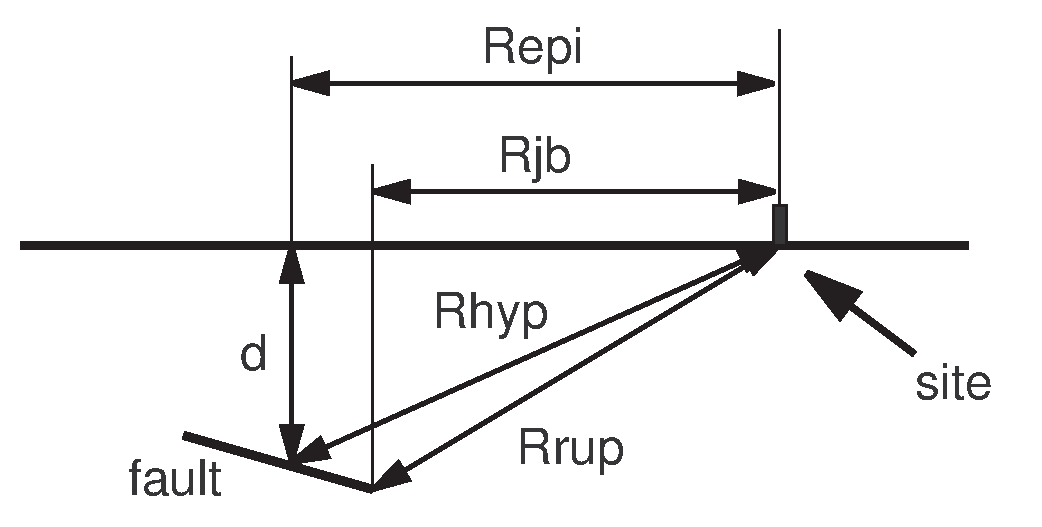
\includegraphics[width=0.7\textwidth]{diags/fig-hattn-distance}
\caption{Diagram showing the distance measures used in various
  attenuation formulae.}
  \label{fig:attn-distances}
\end{figure}
In case of small earthquake that can be represented by a point
source, the point source measures can be considered as
source-to-site distance measure. However, the point source measures
are not suitable to describe the attenuation of ground motion away
from large earthquakes. In this case, the finite source measures are
preferred.

Local site conditions profoundly affect the ground motion record
characteristics. Several numerical and/or empirical techniques have
been proposed to estimate local site responses. Such studies show
distinct amplification levels in the sites of different geological
and geotechnical characteristics; therefore, it is an ordinary
practice to categorize sites into different general classes.
Different sites of the same class are supposed to have local site
responses with similar characteristics. The most commonly used site
categorization schemes by GMPEs are based on geomatrix, surface
geology, and average shear wave velocity over 30m ($V_{S30}$).
Actually, many of the GMPEs follow exactly the same or similar
classification criteria as suggested by the \citet{eqrm_NEHRP00}
(Table ~\ref{NEHRP}). $V_{S30}$ has also been included directly in
the functional form of several GMPEs. It is worth mentioning that in
spite of $V_{S30}$ popularity as a site parameter, it has its own
shortcomings. Several studies have suggested using other site
parameters such as the average shear wave velocity over the depth
equal to a quarter-wavelength of the period of interest
\citep{eqrm_Boore91}, and the average shear wave velocity of
100-200m \citep{eqrm_Lee95}.
\begin{table}[!t]
\renewcommand{\arraystretch}{1.3}
\caption{Site categories in NEHRP provisions} \label{NEHRP}
\centering
\begin{tabular}{|c|c|c|}
\hline
Site Category & Description & $V_{S30}$\\
\hline
A & Hard rock & $>1500 m/s$\\
\hline
B & Firm to hard rock & $760-1500 m/s$\\
\hline
C & Dense soil, soft rock & $360-760 m/s$\\
\hline
D & Stiff soil & $180-360 m/s$\\
\hline
E & Soft clays & $<180 m/s$\\
\hline
\end{tabular}
\end{table}

\section{Implemented GMPEs in EQRM}\label{sec:implemented} In
recent years the number of GMPEs has considerably increased due to
development of strong motion networks and the large number of
available strong motion records. \citet{eqrm_Douglas06} provides a
review on more than 45 GMPEs for the estimation of peak ground
acceleration and 31 GMPEs for the estimation of response spectra.
Generally, GMPEs can be grouped into two different principle
tectonic regions: shallow crustal earthquakes and subduction zone
earthquakes. The shallow crustal earthquakes can be further divided
into earthquakes in active tectonic regions (e.g. Japan, California,
Iran), and earthquakes in stable continental regions (e.g.
Australia, Eastern North America). The subduction zone earthquakes
can be further divided into intraslab events and earthquakes along
the interface of subducting plates (e.g. Japan, Chile, Indonesia).
For details of the main characteristics of each category see
\citet{eqrm_Campbell03}. For each tectonic region, a handful of
GMPEs are available for use within EQRM software. Their main
characteristics are summarized in Table~\ref{GMPEs}. All of these
equations are widely used in engineering and engineering seismology.
They reflect a broad variety of tastes in terms of their functional
forms and databases.

Considering the general tectonic setting of the region of interest,
the user may either select GMPEs from those listed in
Table~\ref{GMPEs}, or implement his or her desirable model. It
should be also noted that GMPEs have to be selected based on their
magnitude and frequency validity ranges. In other words, GMPEs
should not be used outside the ranges of their underlying dataset
\citep{eqrm_Bommer07}. General guidelines on selection of GMPEs for
seismic hazard analysis are provided by \citet{eqrm_Cotton06} and
\citet{eqrm_Bommer10}. In addition, if strong motion data is
available in the target region, it can be used to verify candidate
GMPEs. To compare ground motions or GMPEs between regions, the main
approaches are the direct comparison of median predictions from
GMPEs for different regions \citep{eqrm_Stafford08}, analysis of
variance \citep{eqrm_Douglas04}, and evaluation of the consistency
of data distributions with respect to a GMPE using likelihood
concepts \citep{eqrm_Scherbaum04} or information-theory approach
\citep{eqrm_Scherbaum09}.

The complexity of the implemented GMPEs varies based on the database
size and developers preferences. In Table~\ref{GMPEs}, the
complexity of each GMPE is represented as the number of the
regression coefficients. In addition to magnitude scaling, distance
scaling and local site condition terms, some of the GMPEs have extra
terms to model other phenomena affecting the ground motion
amplitudes. Table ~\ref{terms} lists these terms for GMPEs developed
for active crustal regions. As it can be seen, among the selected
GMPEs, \citet{eqrm_Abrahamson08}, \citet{eqrm_Campbell08}, and
\citet{eqrm_Chiou08} models can be considered as the most complex
with many input parameters required. They notably require extra
input parameters to model: (1) observed higher ground-motions on the
hanging-wall of the fault-plane, (2) larger ground-motions generated
by buried rupture earthquakes, and (3) basin effect which is
believed to have significant impact on amplification of ground
motion especially at longer period range.
\begin{landscape}
\begin{table}
\centering
\renewcommand{\arraystretch}{1.3}
\caption{Main characteristics of the implemented GMPEs}
\label{GMPEs} \centering {\small
\begin{tabular}{|c|c|c|c|c|c|c|c|c|}
\hline  Model &  Magnitude &  Magnitude &  Distance & Distance &
 Site
&  Horizontal Component & Period &  Complexity  \\
 Name &  Type &  Range
&  Type &  Range &  Condition
&  Type &  Range &\\
\hline \multicolumn{9}{|c|}{Shallow crustal events in active
tectonic regions}\\
\hline \citet{eqrm_Sadigh97a} & $M_W$ & 4-7.4 & $R_{rup}$ &
0-100& $GMX$ & Geometric mean & 0-4 & 9\\
\hline  \citet{eqrm_Zhao06} & $M_W$ & 4.9-8.3 & $R_{rup}$ &
0-300& $V_{S30} Class$ & Geometric mean & 0-5 & 16\\
\hline  \citet{eqrm_Abrahamson08} & $M_W$ & 5.0-8.0 &
$R_{jb}$ & 0-200 & $V_{S30}$ & GMRotI50 & 0-10 & 17\\
\hline \citet{eqrm_Boore08} & $M_W$ & 5.0-8.0 &
$R_{rup}$ & 0-200 & $V_{S30}$ & GMRotI50 & 0-10 & 14\\
\hline  \citet{eqrm_Campbell08} & $M_W$ & 4.0-8.5 &
$R_{rup}$ & 0-200 & $V_{S30}$ & GMRotI50 & 0-10 & 17\\
\hline  \citet{eqrm_Chiou08} & $M_W$ & 4.0-8.5 &
$R_{rup}$ & 0-200 & $V_{S30}$ & GMRotI50 & 0-10 & 25\\
\hline \citet{eqrm_Akkar10} & $M_W$ & 5.0-7.6 & $R_{jb}$
& 0-100& $V_{S30}$ Class & Geometric mean & 0-3 & 14\\
\hline \multicolumn{9}{|c|}{Shallow crustal events in stable
continental regions}\\
\hline  \citet{eqrm_Gaull90a} & $M_L$ & 4.5-7.2  &
$R_{hypo}$& 10-500& $V_{S30}$ Class & Random & 0-2 & 4\\
\hline \citet{eqrm_Atkinson97a} & $M_W$ & 4.0-7.25 &
$R_{hypo}$& 10-500& $V_{S30}$ Class & Random & 0-2 & 5\\
\hline \citet{eqrm_Toro97a} & $M_W$ & 5.0-8.0 &
$R_{jb}$& 1-500& Hard Rock & Geometric mean & 0-2 & 9\\
\hline \citet{eqrm_Campbell03a} & $M_W$ & 5.0-8.2 &
$R_{rup}$& 1-1000& Hard Rock & Geometric mean & 0-4 & 13\\
\hline \citet{eqrm_Atkinson06} & $M_W$ & 4.0-8.0 &
$R_{rup}$& 1-1000& $V_{S30}$ & Random & 0-5 & 14 \\
\hline  \citet{eqrm_Liang08} & $M_L$ & 4.0-7.0 &
$R_{epi}$& 10-200& Hard Rock & Random & 0-30 & 6\\
\hline \citet{eqrm_Somerville09} & $M_W$ &5-7.5  &
$R_{jb}$& 0-500& Hard Rock &  Average& 0-10 & 10\\

\hline \multicolumn{9}{|c|}{Subduction zone events}\\
\hline \citet{eqrm_Youngs97} & $M_W$ & 5.0-8.2 &
$R_{rup}$& 10-500& GMX & Geometric mean & 0-3 & 7\\
\hline \citet{eqrm_Atkinson03}& $M_W$ & 5.0-8.3 &
$R_{rup}$& 10-500& $V_{S30}$ Class & Random & 0-3 & 9\\
\hline \citet{eqrm_Zhao06} & $M_W$ & 5.0-8.3 & $R_{rup}$ &
30-300& $V_{S30} Class$ & Geometric mean & 0-5 & 16\\
\hline

\end{tabular}}
\end{table}
\end{landscape}




The above mentioned GMPEs as well as \citep{eqrm_Boore08} model
account for nonlinear site amplification that is due to nonlinear
soil response beyond a certain level of deformations. These models
are developed as part of the Next Generation of Attenuation of
Ground-Motions (NGA) project in 2008 for shallow crustal earthquakes
in California. In many regions, however, it is not possible to
determine all the necessary input parameters for such complicated
models. General guidelines on estimating unknown input parameters
when implementing NGA GMPEs in engineering practice are presented in
\citet{eqrm_Kak11}. The details on how EQRM feeds each of the
implemented GMPEs are given in the next section.
%\begin{landscape}
\begin{table}[!t]
\centering
\renewcommand{\arraystretch}{1.3}
\caption{Functional forms of GMPEs for active tectonic regions}
\label{terms} \centering {\small
\begin{tabular}{c c c c c c c c}
\hline
&\multicolumn{7}{c}{Ground Motion Prediction Equations}\\
\hline
 Term &  Sa97&  Zh06
& AS08& BA08&
 CB08& CY08&  AB10\\
\hline  Near-fault & \multirow{2}{*}{\Checkmark} &
\multirow{2}{*}{\Checkmark}& \multirow{2}{*}{\Checkmark}&
\multirow{2}{*}{\Checkmark}& \multirow{2}{*}{\Checkmark}&
\multirow{2}{*}{\Checkmark}&\multirow{2}{*}{\Checkmark}\\

 Saturation \\

\hline  Magnitude-dependent &
\multirow{2}{*}{\XSolidBrush}&\multirow{2}{*}{\XSolidBrush} &
\multirow{2}{*}{\Checkmark}& \multirow{2}{*}{\Checkmark}&
\multirow{2}{*}{\Checkmark}&
\multirow{2}{*}{\Checkmark}& \multirow{2}{*}{\Checkmark}\\
 Distance Decay \\


\hline  Style of Faulting &{\Checkmark}& {\Checkmark}& {\Checkmark}&
{\Checkmark}& {\Checkmark}&{\Checkmark}&
 {\Checkmark}\\

\hline  Depth-to-Top  &\multirow{2}{*}{\XSolidBrush} &
\multirow{2}{*}{\XSolidBrush}&
\multirow{2}{*}{\Checkmark}&\multirow{2}{*}{\XSolidBrush} &
\multirow{2}{*}{\Checkmark}&\multirow{2}{*}{\Checkmark}&\multirow{2}{*}{\XSolidBrush} \\

 of Rupture\\

\hline  Hanging-Wall &{\XSolidBrush} &{\XSolidBrush} &
{\Checkmark}&{\XSolidBrush} &
{\Checkmark}& {\Checkmark}&{\XSolidBrush} \\

\hline  Basin Effect &{\XSolidBrush} &{\XSolidBrush} &
{\Checkmark}&{\XSolidBrush} &
{\Checkmark}& {\Checkmark}& {\XSolidBrush}\\

\hline  Nonlinear  & \multirow{2}{*}{\XSolidBrush}&
\multirow{2}{*}{\XSolidBrush}& \multirow{2}{*}{\Checkmark}&
\multirow{2}{*}{\Checkmark}&
\multirow{2}{*}{\Checkmark}& \multirow{2}{*}{\Checkmark}&\multirow{2}{*}{\XSolidBrush}\\
Site Response\\
\end{tabular}}
\end{table}
%\end{landscape}



\section{Implementation}\label{sec:implementation} In the EQRM
application the attenuation calculations are conducted within the
main driving function \typefunc{do}{\_ana}{lysis} which computes the
attenuation for one site at a time for all events and all
fundamental (or building) periods. That is, for each site there
exists a large matrix of modelled $S_a(T_o,r_m,R)$ (this matrix is
\typevar{S}{}{A} or \typevar{SA}{ro}{ck} in the code) whose rows
correspond to the events (i.e. an $r_m$-$R$ pair) and whose columns
correspond to the $T_o$. That is

\begin{math}
%\label{fig:attn-sa-matrix}
 SA = \left[ \begin{array}{ccccc}
S_a(T_{o,1},r_{m,1},R_1) & S_a(T_{o,2},r_{m,1},R_1) &  \hdots & S_a(T_{o,N_T},r_{m,1},R_1) \\
S_a(T_{o,1},r_{m,2},R_2) & S_a(T_{o,2},r_{m,2},R_2) &  \hdots & S_a(T_{o,N_T},r_{m,2},R_2) \\
\vdots & \vdots &  \ddots & \vdots \\
S_a(T_{o,1},r_{m,N_s},R_{N_s}) & S_a(T_{o,2},r_{m,N_s},R_{N_s}) & \hdots & S_a(T_{o,N_T},r_{m,N_s},R_{N_s}) \\
\end{array} \right]
\end{math}

where $N_s$ refers to the number of events and $N_T$ refers to the
number of periods. Note that the $r_m$-$R$ pair comes from the event
catalogue and a calculation of distance, as described in this
section. The $T_o$ are determined by the user using the EQRM control
file parameter: \typeself{atten-periods}. Computationally the above
calculation of attenuation is conducted in two parts as follows:
\begin{enumerate}
\item The preparation of the attenuation coefficients
conducted before entering a loop over sites. This preparation
involves interpolating the attenuation coefficients to the
fundamental periods defined by the user. \item The computation of
the $S_a(T_o,r_m,R)$ at each site conducted site-by-site within a
loop over sites. Note that this process is vectorised over the
earthquakes in the synthetic event catalogue.
\end{enumerate}


Each GMPE returns an estimate of:
\begin{enumerate}
\item the mean of $log(S_a(T_o,r_m,R))$ (equivalent to the
logarithm of the median of $S_a(T_o,r_m,R)$) and hereafter denoted
by $\mu_{log(S_a)}(T_o,r_m,R)$ or $\mu_{log(S_a)}$ for brevity, and
\item the standard deviation of $log(S_a(T_o,r_m,R))$, hereafter
denoted by \newline $\sigma_{log(S_a)}(T_o,r_m,R)$ or
$\sigma_{log(S_a)}$ for brevity.
\end{enumerate}


The required input parameters by implemented GMPEs in EQRM, to model
source, path and site effects are listed in Table ~\ref{inputs}. The
abbreviations used in this Table are defined in Table ~\ref{def}. As
it can be seen GMPEs use different definitions for explanatory and
response variables. Regarding response parameter,i.e. ground-motion
parameter of interest, currently EQRM estimates $5 \%$ $S_a$ using
GMPEs listed in Table \ref{GMPEs}. Conversion equations between
different definitions of response variables are provided by
\citet{eqrm_Beyer06}.  For each GMPE, EQRM should provide inputs
respecting the original definition used within each model. In EQRM,
the recurrence relationship and hence the generated earthquake
catalogue are based on moment magnitude scale. However, among the
implemented GMPES \citet{eqrm_Gaull90a}, and \citet{eqrm_Liang08}
models use $M_L$ scale. In this case, adjustment is done using the
correlation relationship between $M_L$ and $M_W$ as suggested by
Johnston (\textit{pers. comm.}, 2001):
\begin{equation}\label{ml-mw}
M_L =
\frac{0.473+\sqrt{0.473^2-4\times0.145(3.45-M_W)}}{2\times0.145};
\end{equation}
Equation~\ref{ml-mw} is developed for stable continental regions and
is based on earlier work published by the same author
\citep{eqrm_Johnstone96a}. It is important to note that
uncertainties in the explanatory variables are map to the response
variable \citep{eqrm_Bommer05}. In other words, in equation
~\ref{eq:general} if an explanatory parameter, $x$, has been
assigned using a correlation conversion with associated measure of
aleatory variability, $\sigma_x$, then this should be map into the
aleatory variability of the GMPEs, $\sigma_y$, by using the
expression:
\begin{equation}
\sigma_{Total} = \sqrt{\sigma_y^2+(\dfrac{\partial log(Y)}{\partial
x})^2 \sigma_x^2}
\end{equation}
Traditionally in seismic hazard studies the most difficult
adjustments are conversions between different source-to-site
distance measures. \citet{eqrm_Scherbaum04b} and later
\citet{eqrm_Kak11} proposed correlation relations among popular
distance metrics. It is important to note that, as indicated by
\citet{eqrm_Scherbaum05}, large penalties can be paid in terms of
increased standard deviation values due to conversion of
source-to-site distance measures. However, in EQRM distance measures
conversions are not necessary, since virtual fault-planes are
generated through simulation process. This enables EQRM to not only
directly calculate the proper Finite-source distance measure for
each GMPE, but also to estimate all the source geometry related
parameters, i. e. $h$, $W$, $\delta$, $R_x$. It should be noted that
\citet{eqrm_Gaull90a}, and \citet{eqrm_Liang08} models use
point-source distance measures: $R_{hypo}$ and $R_{epi}$. There are
two obvious techniques that could be used to approximate $\Repi$ and
$\Rhyp$. The first technique approximates $\Repi$ and $\Rhyp$ using
$\Rjb$ and $\Rrup$ respectively. This technique is conservative
since \mbox{$\Repi \geq \Rjb$} and \mbox{$\Rhyp \geq \Rrup$}. The
second technique involves approximating $\Rhyp$ by using the
distance to the rupture centroid and $\Repi$ with the distance to
the vertical surface projection of the rupture centroid. The EQRM
application currently uses the first (i.e. conservative) technique.

The only remaining parameters to be determined are site parameters.
The $V_{S30}$ parameter is the required INPUT parameter that should
be provided by the user. In the absence of shear-wave velocity
measurements in the target region, several techniques exist to
estimate $V_{S30}$; use of geological maps, geomorphological maps,
topographic slope maps, to name a few. The Z1.0 and Z2.5 parameters
are used by some of the NGA GMPEs to model the basin effects.
Currently these parameters are not included in the INPUT file, and
are estimated as follows: Z1.0 is estimated from Vs30 following the
correlation relation suggested by \citet{eqrm_Chiou08}:
\begin{equation}
ln(Z_{1.0}) = 28.5-0.4775ln(V_{S30}^8+38.7^8)
\end{equation}

Z2.5 is approximated from Z1.0 following the correlation relation
suggested by \citet{eqrm_Campbell07}:
\begin{equation}
ln(Z_{2.5}) = 0.519+3.595Z_{1.0}
\end{equation}
It should be noted that by using these relations, we assume that the
basin depths at target region and California are similar. However if
it would not be the case this may introduce bias in predictions at
longer periods, where the basin effects are most pronounced.

\subsection{Further Comments on Specific GMPEs}

\subsubsection{\citet{eqrm_Gaull90a}}
The \citet{eqrm_Gaull90a} model is based on empirical intensity data
in the Australian region and the PGA extension created using Papua
New Guinea data. For the purpose of this GMPE the Australian region
is divided into four sub-regions, Western Australia, Southeastern
Australia, Northeastern Australia and Indonesia. In the EQRM
application, currently the model for Western Australia (PGA version)
is implemented.

Note that in the case of the \citet{eqrm_Gaull90a} attenuation model
there is no need to prepare the attenuation coefficients because the
attenuation model is only defined for $T_o=0 sec$ (PGA). To compute
$S_a(T_o,r_m,R)$ (more specifically, $\mu_{log(S_a)}$), we can
extend the $PGA$ estimate using the Australian Standard Response
Spectral Acceleration \citep{eqrm_Aus93}.

\citet[Table 4]{eqrm_Gaull90a} tabulate the `uncertainty
parameter(s)' ($\sigma_{log(Y)}$) and indicate that they do not
depend on $r_{m_l}$ or $\Rhyp$. Furthermore, when extending the PGA
estimate to a complete $S_a$ it is assumed that $\sigma_{log(S_a)}$
is not a function of $T_o$, in other words:
\begin{equation}
\sigma_{log(S_a)}(T_o) = \sigma_{log(PGA)}.
\end{equation}
Personal discussions with Brian Gaull (2002 and 2003) have revealed
that the following values of $\sigma_{log(Y)}$; 0.7 (for PGA) and
0.925 (for $\Imm$) should be used in preference to the published
values of 0.28 and 0.37 respectively.
\begin{landscape}
\begin{table}[!t]
\renewcommand{\arraystretch}{1.3}
\caption{Input parameters of the implemented GMPEs in EQRM}
\label{inputs} \centering

{\footnotesize
\begin{tabular}{c c c c c c c c c c c c c c c c c c}
\hline
&\multicolumn{17}{c}{Ground Motion Prediction Equations}\\
\hline
 Parameter & Sa97& Zh06&AS08
 &BA08&CB08&CY08&AB10&
 Ga90& AB97&To97&
 Ca03&AB06&Li08&So09
 &Yo97&AB03&Zh06\\
\hline { Source parameters}\\
$M_L$&&&&&&&&\textbullet&&&&&\textbullet&&&&\\
$M_W$&\textbullet&\textbullet&\textbullet&\textbullet&\textbullet&\textbullet&\textbullet
&&\textbullet&\textbullet&\textbullet&\textbullet&&\textbullet&\textbullet
&\textbullet&\textbullet\\
$h$&&&&&&& &&&&&&&&\textbullet
&\textbullet&\textbullet\\
$Z_{TOR}$&&&\textbullet&&\textbullet&\textbullet& &&&&&&&&
&&\\
$W$&&&\textbullet&&&& &&&&&&&&
&&\\
$\delta$&&&\textbullet&&\textbullet&\textbullet& &&&&&&&&
&&\\
$SOF
Flag$&\textbullet&\textbullet&\textbullet&\textbullet&\textbullet&\textbullet&\textbullet
&&&&&&&&
&&\\
\hline { Path parameters}\\
$R_{epi}$&&&&&&& &&&&&&\textbullet&&
&&\\
$R_{hypo}$&&&&&&& &\textbullet&\textbullet&&&&&&
&&\\
$R_{jb}$&&&\textbullet&\textbullet&\textbullet&\textbullet&\textbullet
&&&\textbullet&&&&\textbullet&
&&\\
$R_{rup}$&\textbullet&\textbullet&\textbullet&&\textbullet&\textbullet&
&&&&\textbullet&\textbullet&&&\textbullet
&\textbullet&\textbullet\\
$R_x$&&&\textbullet&&&\textbullet& &&&&&&&&
&&\\
$HW Flag$&&&\textbullet&&\textbullet&\textbullet& &&&&&&&&
&&\\
\hline { Site parameters}\\
$Site Flag$&\textbullet&\textbullet&&&&&\textbullet
&\textbullet&\textbullet&&&&&&\textbullet
&\textbullet&\textbullet\\
$V_{S30}$&&&\textbullet&\textbullet&\textbullet&\textbullet&
&&&&&\textbullet&&&
&&\\
$Z_{1.0}$&&&\textbullet&&&\textbullet& &&&&&&&&
&&\\
$Z_{2.5}$&&&&&\textbullet&& &&&&&&&&
&&\\
$PGA_{rock}$&&&\textbullet&\textbullet&\textbullet&\textbullet&
&&&&&\textbullet&&&
&&\\
\end{tabular}}
\end{table}
\end{landscape}

\begin{table}[!t]
\renewcommand{\arraystretch}{1.3}
\caption{Definition of Input parameters} \label{def} \centering
\begin{tabular}{|c|c|}
\hline Parameter& Description\\
\hline $M_W$ & {\small Moment magnitude}\\

\hline $M_L$ & {\small Local magnitude}\\

\hline $h$ & {\small Focal depth (km)}\\

\hline $W$ & {\small Down-dip rupture width (km)}\\

\hline $\delta$ & {\small Fault dip (degree)}\\

\hline $SOF$ & {\small Style Of Faulting (function of rake angle,
$\lambda$
(degree))}\\

\hline $R_{epi}$ & {\small Distance from the epicenter (km)}\\

\hline $R_{hypo}$ & {\small Distance from the hypocenter (km)}\\

\hline $R_{jb}$ & {\small Closest distance to the surface projection
of the
rupture plane (km)}\\

\hline $R_{rup}$ & {\small Closest distance to the rupture plane (km)}\\

\hline $R_x$ & {\small Horizontal distance to top edge of rupture}\\
 &{\small measured
perpendicular to the strike (km)}\\

\hline $HW Flag$ & {\small Hanging-Wall Flag}\\

\hline $Site Flag$ & {\small Site Class Flag}\\

\hline $V_{S30}$ & {\small Average shear-wave velocity over the top 30 m (m/s)}\\

\hline $Z_{1.0}$ & {\small Depth to shear-wave velocity equal to 1.0
km/s
(km)}\\

\hline $Z_{2.5}$ & {\small Depth to shear-wave velocity equal to 2.5
km/s
(km)}\\

\hline $PGA_{rock}$ &{\small Peak Ground Acceleration on rock ($cm/s^2$)}\\
\hline

\end{tabular}
\end{table}





\subsubsection{\citet{eqrm_Somerville09}}

The \citet{eqrm_Somerville09} model is derived from broad-band
strong ground motion simulations that use the Non-Cratonic and
Cratonic earthquake source models together with crustal structure
models representing different regions of Australia (\citet[Table
7-1]{eqrm_Somerville09}). Two general models are also developed:
Yilgarn Craton model which is applicable to Yilgarn Craton and other
cratonic regions of Australia, and Non-Cratonic model applicable in
all non-cratonic regions of Australia. For completeness sake, the
model coefficients for Non-Cratonic model is listed in
Table~\ref{tab:Coeff-Somerville09_Non_Cratonic} because it was
omitted from the original publication.

\begin{table}
\caption{Coeeficients for \texttt{Somerville09\_Non\_Cratonic}. The
Non-Cratonic model represents an everage model for all non cratonic
regions of Australia } \label{tab:Coeff-Somerville09_Non_Cratonic}
\footnotesize
\begin{tabular}{ccccccccc}
 \hline
Period  & $C_1$    & $C_2$     & $C_3$     & $C_4$     & $C_5$    & $C_6$    & $C_7$    & $C_8$ \\
\hline
PGA     & 1.03780  & -0.03970  & -0.79430  & 0.14450   & -0.00618 & -0.72540 & -0.03590 & -0.09730 \\
0.010   & 1.05360  & -0.04190  & -0.79390  & 0.14450   & -0.00619 & -0.72660 & -0.03940 & -0.09740 \\
0.020   & 1.05680  & -0.03920  & -0.79680  & 0.14550   & -0.00617 & -0.73230 & -0.03930 & -0.09600 \\
0.030   & 1.13530  & -0.04790  & -0.80920  & 0.15000   & -0.00610 & -0.76410 & -0.05710 & -0.09210 \\
0.040   & 1.30000  & -0.07020  & -0.83150  & 0.15920   & -0.00599 & -0.82850 & -0.09810 & -0.08530 \\
0.050   & 1.47680  & -0.09310  & -0.83330  & 0.15600   & -0.00606 & -0.86740 & -0.12740 & -0.09130 \\
0.075   & 1.70220  & -0.05160  & -0.80720  & 0.14560   & -0.00655 & -0.87690 & -0.10970 & -0.08690 \\
0.100   & 1.65720  & 0.15080   & -0.77590  & 0.13100   & -0.00708 & -0.77830 & 0.01690  & -0.05980 \\
0.150   & 1.94440  & -0.09620  & -0.75000  & 0.11670   & -0.00698 & -0.69490 & -0.13320 & -0.12530 \\
0.200   & 1.82720  & -0.06230  & -0.73430  & 0.11940   & -0.00677 & -0.64380 & -0.09570 & -0.11920 \\
0.250   & 1.74380  & -0.02530  & -0.72480  & 0.11950   & -0.00646 & -0.63740 & -0.06250 & -0.11650 \\
0.3003  & 1.80560  & -0.27020  & -0.73190  & 0.13490   & -0.00606 & -0.66440 & -0.17470 & -0.14340 \\
0.400   & 1.88750  & -0.37820  & -0.70580  & 0.09960   & -0.00589 & -0.58770 & -0.24420 & -0.21890 \\
0.500   & 2.03760  & -0.79590  & -0.69730  & 0.11470   & -0.00565 & -0.59990 & -0.48670 & -0.29690 \\
0.750   & 1.93060  & -0.80280  & -0.74510  & 0.11220   & -0.00503 & -0.59460 & -0.50120 & -0.34990 \\
1.000   & 1.60380  & -0.47800  & -0.86950  & 0.07320   & -0.00569 & -0.41590 & 0.06360  & -0.33730 \\
1.4993  & 0.47740  & 0.90960   & -1.02440  & 0.11060   & -0.00652 & -0.19000 & 1.09610  & -0.10660 \\
2.000   & -0.25810 & 1.37770   & -1.01000  & 0.10310   & -0.00539 & -0.27340 & 1.50330  & -0.04530 \\
3.0003  & -0.96360 & 1.14690   & -0.88530  & 0.10380   & -0.00478 & -0.40420 & 1.54130  & -0.11020 \\
4.000   & -1.46140 & 1.07950   & -0.80490  & 0.10960   & -0.00395 & -0.46040 & 1.41960  & -0.14700 \\
5.000   & -1.61160 & 0.74860   & -0.78100  & 0.09650   & -0.00307 & -0.46490 & 1.24090  & -0.22170 \\
7.5019  & -2.35310 & 0.35190   & -0.64340  & 0.09590   & -0.00138 & -0.68260 & 0.92880  & -0.31230 \\
10.000  & -3.26140 & 0.69730   & -0.62760  & 0.12920   & -0.00155 & -0.61980 & 1.01050  & -0.24550 \\
PGV     & 5.07090  & 0.52780   & -0.85740  & 0.17700   & -0.00501 & -0.61190 & 0.80660  & -0.03800 \\
\hline
\end{tabular}
\end{table}


\normalsize



\section{Accounting for uncertainties}\label{sec:uncertain}
Incorporating uncertainty is a critical component of any PSHA.
Regarding GMPEs, seismic hazard studies incorporate two types of
uncertainty: aleatory variability and epistemic uncertainty. By
definition, aleatory variability is the natural random variation of
observed ground-motions with respect to explanatory variables that
cannot be reduced with increasing knowledge about the earthquake
process. It is worth to mention that the aleatory variability can
not be reduced with respect to a particular model, however in
practice it is desirable to reduce the aleatory variability
\citep{eqrm_Atik10}. The aleatory variability is represented by the
standard deviation of the PDF for the GMPEs. Epistemic uncertainty
is the uncertainty raised from our lack of knowledge about
earthquake process. With increased data and knowledge, ideally, the
epistemic uncertainty can be reduced to zero. The epistemic
uncertainty is represented by means of logic-tree. In logic-tree
approach, several GMPEs would be considered, and each equation is
assigned a weighting factor that is interpreted as the relative
likelihood of that equation being correct. It should be noted that
selection of proper ground motion models has stronger influence on
the final results than assigning weights to each model
\citep{eqrm_Scherbaum05}. The incorporation of aleatory variability
and epistemic uncertainty in EQRM are discussed in
~\sref{attn:uncertainty} and ~\sref{sec:attn-multi-attnmodels}
respectively.




\section{Incorporating aleatory variability}
\label{attn:uncertainty}

The aleatory variability is based on estimations of
$\sigma_{log(S_a)}$ (see ~\sref{sec:uncertain}) as provided by GMPEs
developers.
\sreftwo{attn:uncert-randomchoice}{attn:uncert-pdfchoice} describe
two of the most commonly used techniques for incorporating aleatory
variability when using the EQRM. The flag to control the variability
method is \typepar{atten}{\_variability}{\_method}(see
~\sref{sec:application-EQRMcf}).

\subsection{Random sampling of a response spectral acceleration\index{response spectral acceleration}}
\label{attn:uncert-randomchoice}

This technique involves selecting a single `random' response
spectral acceleration\index{response spectral acceleration} ($S_a$)
from its PDF by:
\begin{enumerate}
\item Selecting a random number $n_{rand}$ from the standard
normal distribution $ N \sim (0,1)$. \item Computing the $S_a$ as
follows
\begin{equation}
\label{attn:attn-var} log(A_{S_a}(T_o,r_m,R)) = \mu_{log(S_a)} +
n_{rand} \sigma_{log(S_a)},
\end{equation}
where $\sigma_{log(S_a)}$ is usually assumed to be $\sigma_a$.
\end{enumerate}

\begin{figure}
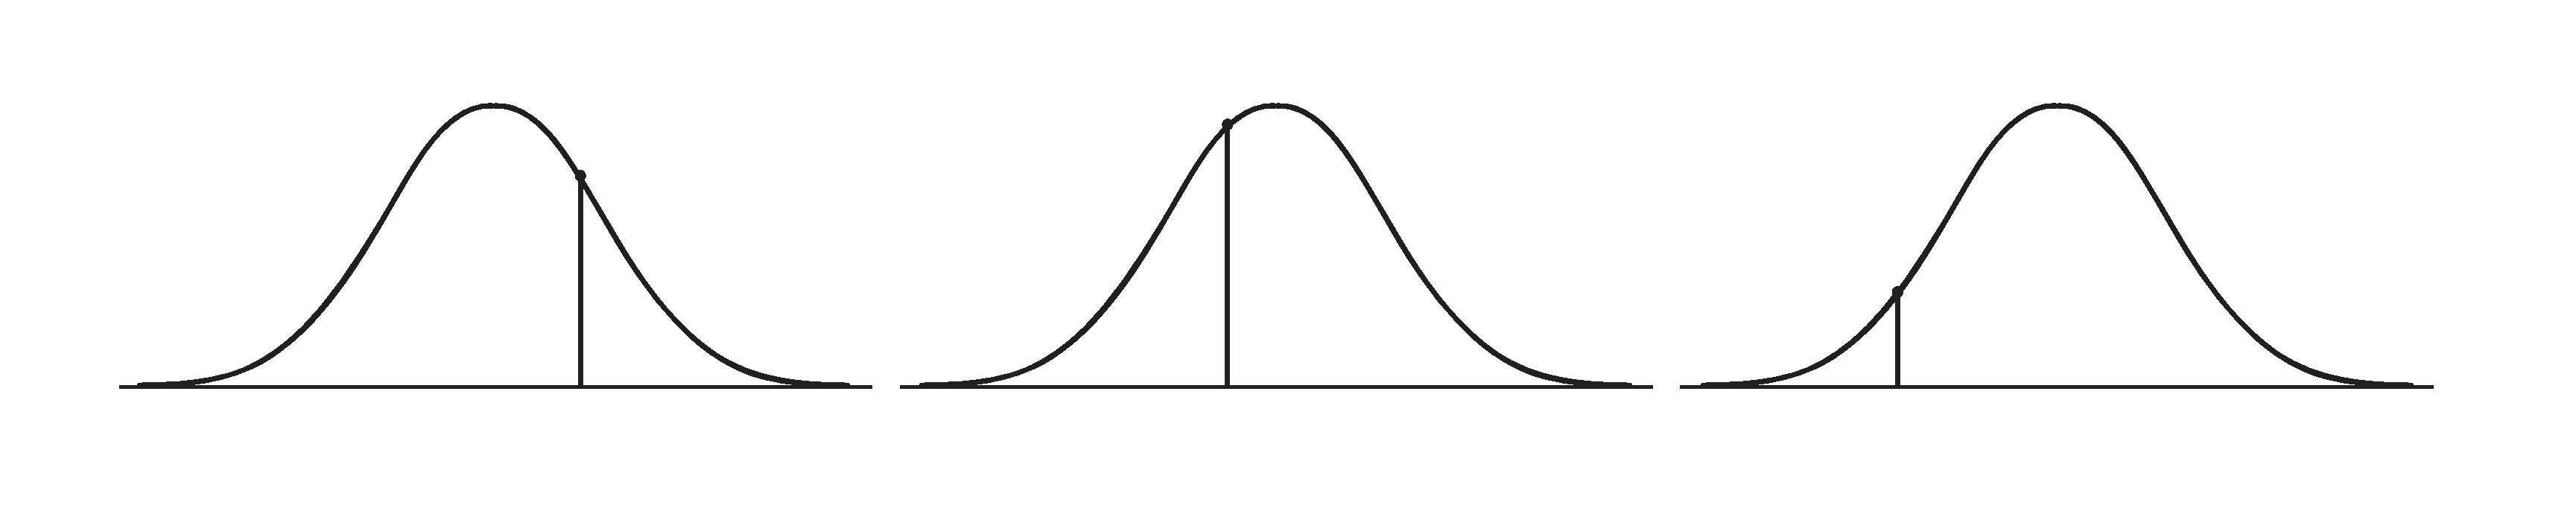
\includegraphics[width=1\textwidth]{diags/fig-hattn-random}
\caption{Selection of three different random samples from a PDF.}
\label{fig:hattn-randomsamp}
\end{figure}
Random sampling from a PDF is illustrated in
\fref{fig:hattn-randomsamp}. It is important to note the following
about random selection:
\begin{enumerate}
\item Two sites that are close to one another may give
dramatically different estimates of ground motion for the same
event. Earthquake hazard and risk values that are computed using
random sampling exhibit a low level of spatial correlation.
\item
The number $n_{rand}$ can theoretically take on any value between
$\pm \infty$. Therefore it is possible that estimates of $S_a$ using
\eref{attn:attn-var} can be unrealistically large. The EQRM
overcomes this problem by introducing a scaling factor
$PGA_{cut}=$\typepar{atten}{\_pga}{\_scaling\_cutoff} which is
applied to the RSA as follows:
\begin{equation}
 log(A_{S_a,new}(T_o,r_m,R)) = R_{scale} \times
log(A_{S_a,old}(T_o,r_m,R))
\end{equation}
where
\begin{equation}\label{rw}
R_{scale}  =
\begin{cases}
1,  PGA \leq PGA_{cut}\\
\frac{PGA_{cut}}{log(A_{S_a}(0,r_m,R))},
PGA > PGA_{cut}\\
\end{cases}
\end{equation}

%if PGA > \typepar{atten}{\_pga}{\_scaling\_cutoff}\\
%R_{scale} =
%\frac{\textrm{\typepar{atten}{\_pga}{\_scaling\_cutoff}}}{log(A_{S_a}(0,r_m,R))}
%\\
% log(A_{S_a,new}(T_o,r_m,R)) = R_{scale} \times
%log(A_{S_a,old}(T_o,r_m,R)).
%\end{equation}
\item There is no effort to account for the likelihood (or
probability) of selecting a particular $n_{rand}$ i.e. a particular
value of the $S_a$ is not weighted against its likelihood. It can be
argued that if enough earthquakes are simulated a range of different
$n_{rand}$ will be taken (high and low) and the overall hazard
and/or risk values will converge to the true ones.
\end{enumerate}


\subsection{Sampling the probability density function of
the response spectral acceleration\index{response spectral
acceleration} (spawning)} \label{attn:uncert-pdfchoice}


An alternative technique for incorporating uncertainty relies on
sampling the PDF of the $S_a$. This technique is used by Aon Re
(Mendez, \textit{pers. comm.}, 2003) and is often referred to as
spawning. An integral component of sampling the PDF is the spawning
of events with the event catalogue (see \sref{source:spawning}).
Essentially the approach involves taking a user defined number of
copies of each event. Every event copy is then available for
calculation of hazard (or risk) using a different sample from the
attenuation PDF.
\begin{enumerate}
\item Firstly the user must define a lower magnitude bound
$m_{bnd}$, a number of samples $n_{smples}$ and a PDF range
$n_\sigma$ (see \sref{source:spawning} for a complete definition).
Recall that \typefunc{fuse}{\_4}{hzd} redefines the event activity
$r_\nu$ using a weight $w_e$, derived by truncating and
re-normalising a standard normal distribution to $\pm n_\sigma$.
\item The $S_a$ is computed as follows
\begin{equation}
\label{attn:uncertainty-pdfsample}
\begin{array}{ll}
log(A_{S_a,i}(T_o,r_m,R)) = \mu_{log(S_a)} - \epsilon_i
\sigma_{log(S_a)}\ & \textrm{for $i=1 \ldots
n_{smples}$} \\
\end{array}
\end{equation}
where
\begin{equation}
\label{attn:uncertainty-def-epsilon}
\begin{array}{ll}
\epsilon_i = -n_\sigma + + (i-1)\Delta &
\textrm{for $i=1 \ldots n_{smples}$} \\
\end{array}
\end{equation}
and
\begin{equation}
\Delta = \frac{2n_\sigma}{n_{smples}-1}.
\end{equation}
Note that
\ereftwo{attn:uncertainty-pdfsample}{attn:uncertainty-def-epsilon}
ensure that the $S_a$ associated with each of the event copies are
evenly spread across the domain of the attenuation PDF
(\fref{fig:hattn-spawnsamp}). Recall from \sref{source:spawning}
that the event activities $r_\nu$ giving rise to each of the $S_a$
described in \eref{attn:uncertainty-pdfsample} are modified by
\typefunc{fuse}{\_4}{hzd} as follows:
\begin{equation}
r_{\nu,i} = r_{\nu,original} \times w_{e,i}
\end{equation}
\end{enumerate}

For example, assume that there is an event with $r_\nu=0.05$ that
gives rise to \mbox{$\mu_{log(S_a)}=[0.3g, 0.5g, 0.2g]$} at the
periods \mbox{$T_o = [0s,0.3s,1s]$} respectively. Also assume that
the estimates of $\mu_{log(S_a)}$ have the following standard
deviations \mbox{$\sigma_{log(S_a)}=\sigma_a = [0.03,0.04,0.01]$}.
Defining $m_{bnd}=0$, $n_{smples}=5$ and $n_\sigma=2.5$ gives
\begin{equation}
\Delta = \frac{2 \times 2.5}{5-1} = 1.25,
\end{equation}

and

%%%========================
% Automatically generated by *\diags\make_spawn_table.m
\begin{center} $ \begin{array}{ccccc}
i & w_{e,i} & \epsilon_i & r_\nu & log(A_{S_a,i}) \\
\hline
1 & 0.0219 & -2.5 & 0.0011 & [0.225g, 0.4g, 0.175g] \\
2 & 0.2285 & -1.25 & 0.0114 & [0.2625g, 0.45g, 0.1875g] \\
3 & 0.4991 & 0 & 0.025 & [0.3g, 0.5g, 0.2g] \\
4 & 0.2285 & 1.25 & 0.0114 & [0.3375g, 0.55g, 0.2125g] \\
5 & 0.0219 & 2.5 & 0.0011 & [0.375g, 0.6g, 0.225g] \\
\hline
\end{array}$
\end{center}
%%%========================

\begin{figure}
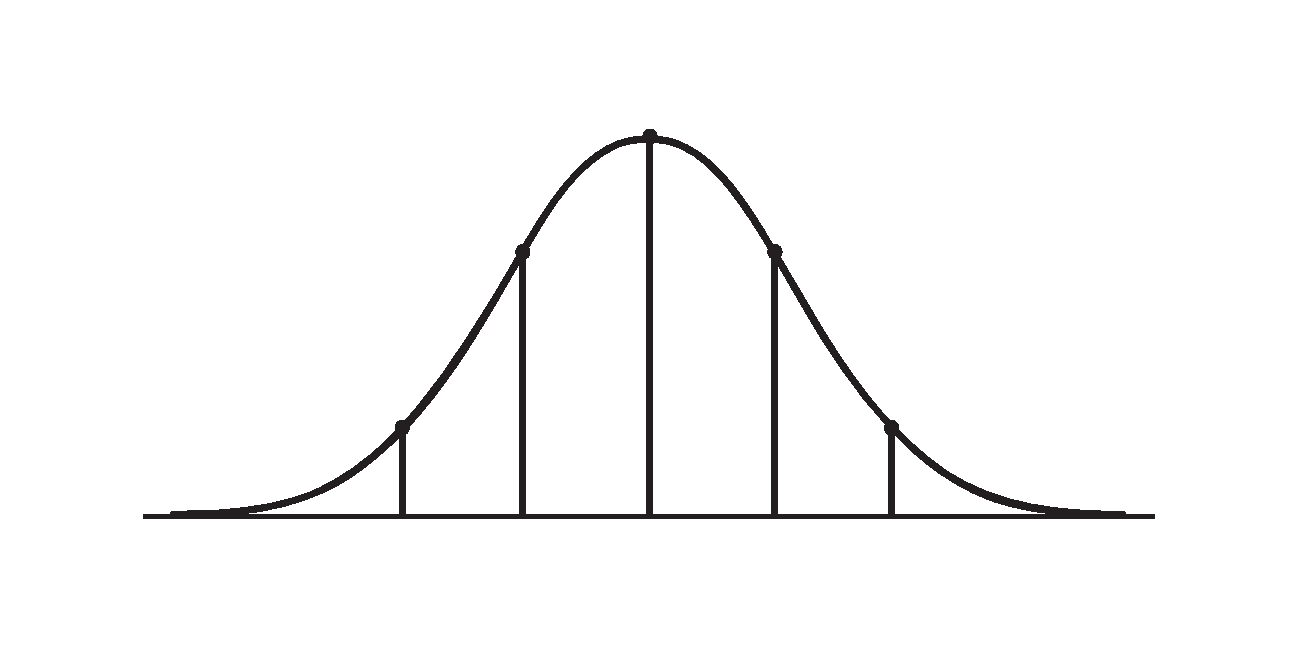
\includegraphics[width=1\textwidth]{diags/fig-hattn-spawning}
\caption{Samples drawn from a PDF using the sampling by spawning
technique with $n_{smples}=5$ and $n_\sigma=2.5$. The width between
the vertical bars is $\Delta$. Note that there is one sample for
each of the five (spawned) copies of the original event.}
\label{fig:hattn-spawnsamp}
\end{figure}

It is important to note the following about spawning:
\begin{enumerate}
\item Sub-sampling the PDF provides a smoother (and repeatable)
estimate of the $S_a$ than random selection
(\sref{attn:uncert-randomchoice}). \item The range of possible $S_a$
values is bounded by the $n_\sigma$. \item Estimates of all $S_a$
are weighted against an event activity $r_\nu$ that accounts for the
likelihood of a particular ground motion being observed. \item The
nature of spawning means that there are more evaluations of the
GMPE. This means that it is typically slower and more memory
intesive since the $S_a$ array is larger.
\end{enumerate}




\subsection{Recomendation for sampling GMPE aleatory Variability}

\textbf{David to complete this section}
\begin{itemize}
\item use spawning for hazard - exaplin why
\item use random sampling for risk - exaplain why
\end{itemize}

\section{Using multiple GMPEs - Incorporating epistemic uncertainty}
\label{sec:attn-multi-attnmodels}

The use of attenuation models in the EQRM is controlled by the
\typeself{set}{da}{ta} parameter \typepar{atten}{uation}{\_flag}.
Recall from \sref{sec:application-setdata} that
\typepar{atten}{uation}{\_flag} is a two row matrix with one column
for each attenuation model to be used. The format of
\typepar{atten}{uation}{\_flag} is
\begin{center}
\begin{math}
%\label{fig:attn-sa-matrix}
 \left[ \begin{array}{ccccc}
P_1 & P_2 &  \hdots & P_n \\
w_{a,1} & w_{a,2} &  \hdots & w_{a,n} \\
\end{array} \right],
\end{math}
\end{center}
where the integers $\{P_i\}_{i=1}^n$ are pointers to the attenuation
model (see \tref{tab:attn-flags}) and the real numbers
$\{w_{a,i}\}_{i=1}^n$ are weights for the respective attenuation
models. Note that the weights $w_i$ must either be all positive or
all negative and
\begin{equation}
\left|\sum_{i=1}^{n}w_{a,i}\right| = 1.
\end{equation}



The mechanism for using more than one attenuation model is similar
to the mechanism used for spawning (see
\sref{attn:uncert-pdfchoice}). That is, the event catalogue is
copied $n$ times (once for each attenuation model) and the
appropriate attenuation model applied to its respective copy. The
values of ground motion (loss for risk) can then be treated
independently for the hazard/risk calculation (if
$\sum_{i=1}^{n}w_{a,i} = -1$) or aggregated before the hazard/risk
assessment is undertaken (if $\sum_{i=1}^{n}w_{a,i} = 1$). This
notion of logic tree collapse is described by
\fref{fig:attn-treecollapse}.


\section{Collapse versus no-collapse}

The techniques adopted for incorporating spawning (see \sref
{attn:uncert-pdfchoice}) and using multiple ground motion models are
similar in the sense that they require multiple evaluations of
ground motion for each event. These are carried through the various
stages of an EQRM simulation such as amplification, building damage
and loss calculation (see following chapters). At the end of the
simulation these values can then be collapsed back to a single `best
estimate' or kept in a un-collapsed form and used to determine the
hazard and/or risk curve (see \cref{ch:risk}). These two options are
illustrated in \fref{fig:attn-treecollapse} for both a hazrd and
risk simulation. Note that when collapsing the samples the extreme
values are removed from the hazard or risk curves. For this reason
we recomend the no-collapse option.

\begin{figure}
 \setlength{\unitlength}{1mm}
(a)  % This is the hazard tree for multi attenuation with collapse

\hspace{4em} \begin{centering}
\begin{picture}(70,30)
% middle branch
\put(0,12){$E_{ij}$} \put(7,13){\vector(1,0){15}}
\put(24,12){$Sa_{ij}^{(2)}$} \put(33,13){\vector(1,0){15}}
\put(50,12){$\widetilde{Sa_{ij}^{(2)}}$} \put(12,14){$w_2$}
% upper branch
\put(7,14){\vector(3,2){15}} \put(24,23){$Sa_{ij}^{(1)}$}
\put(33,24){\vector(1,0){15}}
\put(50,23){$\widetilde{Sa_{ij}^{(1)}}$}
\put(11,20){\rotatebox{30}{$w_1$}}
% lower branch
\put(7,12){\vector(3,-2){15}} \put(24,0){$Sa_{ij}^{(3)}$}
\put(33,1){\vector(1,0){15}} \put(50,0){$\widetilde{Sa_{ij}^{(3)}}$}
\put(11,5){\rotatebox{-30}{$w_3$}}
% concatenation at end
\put(61,5){\scalebox{1.2}[6.5]{\}}} \put(65,12){$ {\displaystyle
\widetilde{Sa_{ij}} = \sum_{k=1}^{3}w_k\widetilde{Sa_k} } $}
\end{picture}
\end{centering}

\vspace{0.8em}
(b) % This is the hazard tree for multi attenuation with NO collapse

\hspace{4em} \begin{centering}
\begin{picture}(70,30)
% middle branch
\put(0,12){$E_{ij}$} \put(7,13){\vector(1,0){15}}
\put(24,12){$Sa_{ij}^{(2)}$} \put(33,13){\vector(1,0){15}}
\put(50,12){$\widetilde{Sa_{ij}^{(2)}}$} \put(12,14){$w_2$}
% upper branch
\put(7,14){\vector(3,2){15}} \put(24,23){$Sa_{ij}^{(1)}$}
\put(33,24){\vector(1,0){15}}
\put(50,23){$\widetilde{Sa_{ij}^{(1)}}$}
\put(11,20){\rotatebox{30}{$w_1$}}
% lower branch
\put(7,12){\vector(3,-2){15}} \put(24,0){$Sa_{ij}^{(3)}$}
\put(33,1){\vector(1,0){15}} \put(50,0){$\widetilde{Sa_{ij}^{(3)}}$}
\put(11,5){\rotatebox{-30}{$w_3$}}
\end{picture}
\end{centering}

\vspace{0.8em}
(c) % This is the risk tree for multi attenuation with collapse

\hspace{4em} \begin{centering}
\begin{picture}(70,30)
% middle branch
\put(0,12){$E_{ij}$} \put(7,13){\vector(1,0){15}}
\put(24,12){$Sa_{ij}^{(2)}$} \put(33,13){\vector(1,0){15}}
\put(50,12){$\widetilde{Sa_{ij}^{(2)}}$} \put(12,14){$w_2$}
\put(60,13){\vector(1,0){15}} \put(77,12){$L_{ij}^{(2)}$}
% upper branch
\put(7,14){\vector(3,2){15}} \put(24,23){$Sa_{ij}^{(1)}$}
\put(33,24){\vector(1,0){15}}
\put(50,23){$\widetilde{Sa_{ij}^{(1)}}$}
\put(11,20){\rotatebox{30}{$w_1$}} \put(60,24){\vector(1,0){15}}
\put(77,23){$L_{ij}^{(1)}$}
% lower branch
\put(7,12){\vector(3,-2){15}} \put(24,0){$Sa_{ij}^{(3)}$}
\put(33,1){\vector(1,0){15}} \put(50,0){$\widetilde{Sa_{ij}^{(3)}}$}
\put(11,5){\rotatebox{-30}{$w_3$}} \put(60,1){\vector(1,0){15}}
\put(77,0){$L_{ij}^{(3)}$}
% concatenation at end
\put(86,5){\scalebox{1.2}[6.5]{\}}} \put(90,12){$ {\displaystyle
 L_{ij} = \sum_{k=1}^{3}w_kL_k } $}
\end{picture}
\end{centering}

\vspace{0.8em}
(d)  % This is the risk tree for multi attenuation with NO collapse


\hspace{4em}\begin{picture}(70,30)
\begin{centering}
% middle branch
\put(0,12){$E_{ij}$} \put(7,13){\vector(1,0){15}}
\put(24,12){$Sa_{ij}^{(2)}$} \put(33,13){\vector(1,0){15}}
\put(50,12){$\widetilde{Sa_{ij}^{(2)}}$} \put(12,14){$w_2$}
\put(60,13){\vector(1,0){15}} \put(77,12){$L_{ij}^{(2)}$}
% upper branch
\put(7,14){\vector(3,2){15}} \put(24,23){$Sa_{ij}^{(1)}$}
\put(33,24){\vector(1,0){15}}
\put(50,23){$\widetilde{Sa_{ij}^{(1)}}$}
\put(11,20){\rotatebox{30}{$w_1$}} \put(60,24){\vector(1,0){15}}
\put(77,23){$L_{ij}^{(1)}$}
% lower branch
\put(7,12){\vector(3,-2){15}} \put(24,0){$Sa_{ij}^{(3)}$}
\put(33,1){\vector(1,0){15}} \put(50,0){$\widetilde{Sa_{ij}^{(3)}}$}
\put(11,5){\rotatebox{-30}{$w_3$}} \put(60,1){\vector(1,0){15}}
\put(77,0){$L_{ij}^{(3)}$}
\end{centering}
\end{picture}


\caption{The application of spawning to a single synthetic
earthquake $E_{ij}$;(a) the collapse of spawned samples for hazard
(\typeparcaption{src}{\_eps}{\_switch}$=1$); (b) hazard spawning
without collapse (\typeparcaption{src}{\_eps}{\_switch}$=2$); (c)
the collapse of spawned samples for risk
(\typeparcaption{src}{\_eps}{\_switch}$=1$); and (d) risk spawning
without collapse (\typeparcaption{src}{\_eps}{\_switch}$=2$). The
illustrated procedure is repeated for $N_s$ events in the event
catalogue and the techniques of \cref{ch:risk} used to assess the
hazard or risk.} \label{fig:attn-treecollapse}
\end{figure}




%%% Local Variables:
%%% mode: latex
%%% TeX-master: "eqrmtech"
%%% End:
